% ++++++++++++++++++++++++++++++++++++++++
% Don't modify this section unless you know what you're doing!
\documentclass[a4paper,12pt]{article}
\usepackage{tabularx} % extra features for tabular environment
\usepackage{amsmath}  % improve math presentation
\usepackage{graphicx} % takes care of graphic including machinery
\usepackage[margin=0.75in]{geometry} % decreases margins
\usepackage{subcaption}
\usepackage{verbatim}
\usepackage{float}
\usepackage{hyperref}
\usepackage{titling}
\hypersetup{
	colorlinks=true,       % false: boxed links; true: colored links
	linkcolor=black,        % color of internal links
	citecolor=blue,        % color of links to bibliography
	filecolor=magenta,     % color of file links
	urlcolor=blue         
}
%++++++++++++++++++++++++++++++++++++++++
\setlength{\parindent}{0pt}
\setlength\parskip{0.5em plus 0.1em minus 0.2em}
\setlength{\droptitle}{-5em}   % This is your set screw

\begin{document}
\title{Charge to Mass Ratio for Electron \\
\large PHY224 Fall 2021}
\author{Fredrik Dahl Bråten, Pankaj Patil}
\date{\today}
\maketitle
\begin{center}
	\section*{Abstract}
\end{center}

In this variation of J. J. Thomson experiment, we aim to estimate the charge to mass ratio of an electron.
As predicted by the theory, we observe the deflection of moving charge in a magnetic field. The electron 
is deflected in such a way that it forms a circular trajectory, for which the radius can be measured. This
radius can then be used to measure the charge to mass ratio for an electron with the help of theoretical formulas
relating the magnetic field to the radius of the orbit. 

\section{Introduction}

\subsection*{A. Background Theory}

Electron moving with velocity $\vec{v}$ through a magnetic field $\vec{B}$, experiences a force $\vec{F} = e\vec{v}\times \vec{V}$.
For constant magnetic field and velocity perpendicular to it, the electron moves in circular orbit, such that $evB = m\frac{v^2}{r}$.

When electron is accelerated through potential $V$, we have $eV = \frac{1}{2}mv^2$, which when combined with former 
equation gives $\frac{1}{r} = \sqrt{\frac{e}{2m}} \frac{B}{\sqrt{V}}$.

By measuring the potential, magnetic field and the radius of the orbit, we can determine the charge to mass ratio with above formula. 

\subsection*{B. Materials and Methods}

The main apparatus for the experiment consists of two Helmholtz coils to produce magnetic field and a vacuum tube to observe electron 
trajectory. 

We followed the instructions given in the lab manual \cite{lab-manual-ex8}, and also the instruction given to us by the TA.

\section{Results}

To compute the external magnetic field, we use $\frac{1}{r} = \sqrt{\frac{e}{2m}}\frac{1}{\sqrt{V}}(B_c + B_e) \implies B_c = (constant)\frac{1}{r} - B_e$. 
The constant factor is due to measurements done with constant voltage. The intercept of the fitted line gives $B_e = 0.00001 \pm 0.00005$ Tesla.

\begin{figure}[H]
  \centering
  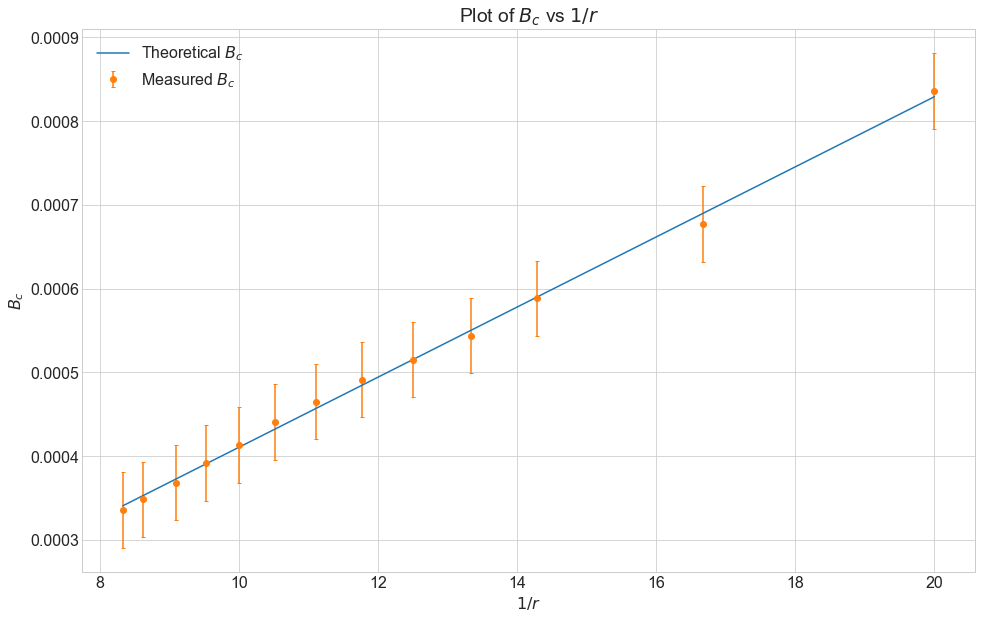
\includegraphics[width=0.8\linewidth]{../code/Pankaj/Coil B vs r_1.png} 
  \begin{center}
    Fitting Equation $f(x) = ax+b$ \\
    $B_e = -b$
  \end{center}  
    \caption{Computation of External Magnetic Field: $B_c$ vs $1/r$}
    \label{b_e}
\end{figure}

To compute the charge to mass ratio we use $\frac{1}{r} = \sqrt{\frac{e}{m}}k\frac{I-I_0}{\sqrt{V}}$. For this case we use the data
obtained keeping current constant. The charge to mass ratio is give by $(\frac{slope}{k(I-I_0)})^2$. The charge to mass ratio
obtained in our case is $-(1.61 \pm 0.04) \times 10^{11}\ C/kg$.

\begin{figure}[H]
  \centering
  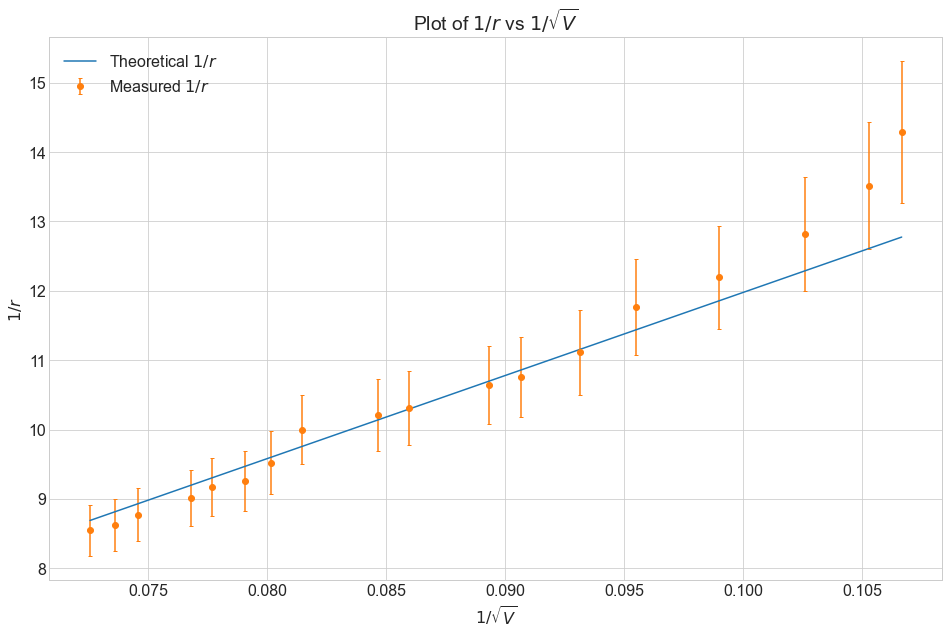
\includegraphics[width=0.8\linewidth]{../code/Pankaj/Charge To Mass Ratio.png}   
  \begin{center}
    Fitting Equation $f(x) = ax$ \\
    $a = 119.77$
  \end{center}   
  \caption{Computation of e/m: $1/r$ vs $1/\sqrt{V}$}
  \label{e_m}
\end{figure}

\section{Uncertainty}

For the calculation of $B_e$, the uncertainty is given by the fitting function. Hence $\Delta B_e = \Delta (y-intercept) = \pm 0.00005$ Tesla.

For the computation of charge to mass ratio, we have $\frac{e}{m} = (\frac{slope}{k(I-I_0)})^2 \implies 
\Delta (\frac{e}{m}) = 2 (slope) \frac{\Delta (slope)}{(k(I-I_0))^2}$. The uncertainty is then $\Delta (\frac{e}{m}) = 0.04 \times 10^{11}\ C/kg$.

\section{Discussion}
 

\pagebreak

\appendix

\section{Appendix}

\subsection{Experimental Data}

\subsubsection*{A Constant Current}

\noindent\rule{\textwidth}{1pt}
\verbatiminput{../data/Changing_voltage.csv}
\noindent\rule{\textwidth}{1pt}

\subsubsection*{B Constant Voltage}

\noindent\rule{\textwidth}{1pt}
\verbatiminput{../data/Changing_current.csv}
\noindent\rule{\textwidth}{1pt}

\pagebreak

\subsection{Python Code}

The Python code for this exercise is divided into two files. statslab.py file contains utility methods
which we will be frequently using in this course. lab\_8.py file contains the code which analyzes
the data.

\subsubsection{statslab.py}
\noindent\rule{\textwidth}{1pt}
\verbatiminput{../code/Pankaj/statslab.py}
\noindent\rule{\textwidth}{1pt}

\pagebreak

\subsubsection{lab\_8.py}
\noindent\rule{\textwidth}{1pt}
\verbatiminput{../code/Pankaj/lab_8.py}
\noindent\rule{\textwidth}{1pt}


\pagebreak

\begin{thebibliography}{99}

\bibitem{lab-manual-ex8} Charge to mass ratio for electron (e/m) - charge\_to\_mass.pdf (\url{https://q.utoronto.ca/courses/235154/files/15436313/download?wrap=1}).

\end{thebibliography}
  
  
\end{document}
